\documentclass[11pt, a4paper]{article}

\usepackage[margin=2.1cm]{geometry}
\usepackage[utf8]{inputenc}
\usepackage[T1]{fontenc}
\usepackage[spanish]{babel}
\usepackage{array}
\usepackage{booktabs}
\usepackage{caption}
\usepackage{float}
\usepackage{graphicx}
\usepackage{hyperref}
\usepackage{xcolor}

\definecolor{cjcblue}{RGB}{31,97,169}

\setlength{\parindent}{0pt}
\setlength{\parskip}{6pt}
\setlength{\textfloatsep}{10pt plus 2pt minus 2pt}
\setlength{\floatsep}{8pt plus 2pt minus 2pt}
\renewcommand{\arraystretch}{1.08}
\captionsetup{font=normalsize, labelfont=bf}
\graphicspath{{Paper/figures/}{figures/}}
\hypersetup{colorlinks=true, urlcolor=cjcblue, linkcolor=black}
\addto\captionsspanish{\renewcommand{\tablename}{Cuadro}}

\begin{document}

\begin{center}

\includegraphics[width=0.30\textwidth]{logo_cjc_palatino_horizontal.png}

\textbf{Comunicado de prensa}

Centro Javeriano de Competitividad \textbar{} Pontificia Universidad Javeriana
\end{center}

{\color{cjcblue}\rule{\textwidth}{0.8pt}}

\begin{center}
{\Large\bfseries Colombia creció más por tener más ocupados que por aumentar su productividad entre 2010 y 2025}

\vspace{4pt}

\textbf{Un informe del Centro Javeriano de Competitividad alerta sobre la caída en la productividad laboral de sectores clave de la economía.}
%\textbf{Un informe del Centro Javeriano de Competitividad muestra que entre 2010 y 2025 el PIB real creció 3,2\% anual, pero el PIB por trabajador aumentó apenas 1,1\% anual.}

Bogotá, 9 de junio de 2026.

\end{center}

%\textbf{Colombia aumentó su PIB por trabajador apenas el 1,1\% anual entre 2010 y 2025.} 
Un nuevo informe del \textbf{Centro Javeriano de Competitividad} muestra que el crecimiento del país provino más de la expansión del número de ocupados que de un aumento del producto por trabajador. %\textbf{La productividad importa porque el ingreso por habitante depende cada vez más de lo que produce cada trabajador.} El ingreso por habitante puede descomponerse entre la proporción de la población que trabaja y lo que produce cada trabajador. En un país que envejece como Colombia, la proporción de la población que trabaja tiende a disminuir. Por lo tanto, el aumento del ingreso por habitante dependerá cada vez más de aumentar el PIB por trabajador.
%\textbf{La productividad importa porque el ingreso promedio de cada habitante de un país es proporcional a lo que produce cada trabajador.} El ingreso por habitante puede descomponerse entre la proporción de la población que trabaja y lo que produce cada trabajador. En un país que envejece como Colombia, la proporción de la población que trabaja tiende a disminuir. Por lo tanto, el aumento del ingreso por habitante dependerá cada vez más de aumentar el producto por trabajador.
El informe, titulado \textbf{Dinámicas de la Productividad Laboral por Actividad Económica en Colombia 2010--2025}, calcula la evolución del \textbf{producto por trabajador} y del \textbf{producto por hora trabajada}, tanto para el agregado nacional como para las principales ramas de actividad económica. %En la medida en que cambian las horas trabajadas por ocupado, ambas medidas pueden evolucionar a ritmos distintos.

\textbf{Entre 2010 y 2025, el número de personas ocupadas aumentó 2,1\% anual, mientras que el PIB por trabajador creció 1,1\% anual.} Por lo tanto, cerca de dos de los poco más de tres puntos porcentuales de crecimiento anual del PIB se explican por el aumento de la población ocupada y el resto por el aumento del producto por trabajador.

\textbf{En el mismo periodo, el PIB por hora trabajada creció 1,5\% anual, pero las horas semanales promedio por trabajador disminuyeron 0,5\% anual.} Esa caída en las horas trabajadas explica por qué el PIB por trabajador creció menos que el PIB por hora trabajada. Por lo tanto, parte de la ganancia en productividad por hora se tradujo en más tiempo disponible fuera del trabajo, una mejora de bienestar que no queda capturada por el aumento de los ingresos.

\textbf{La caída de las horas trabajadas enmascara la contribución del aumento de la productividad por hora al crecimiento del PIB.} El crecimiento anual del PIB real (3,2\%) se explica por el aumento de los ocupados (2,1\%), la caída en las horas trabajadas por ocupado (-0,5\%) y el crecimiento del PIB por hora trabajada (1,5\%). Esta descomposición se resume en la Figura \ref{fig:comunicado_descomposicion}.

\textbf{El informe alerta sobre la caída de la productividad en de varias actividades económicas.} En crecimiento del PIB por trabajador, las tres actividades con mayores aumentos fueron: 1. arte, recreación y otros servicios (7,3\% anual); 2. información y comunicaciones (3,7\%); y 3. agropecuario (2,8\%). En contraste, las tres mayores caídas se registraron en: 1. servicios públicos (-3,8\% anual); 2. minas (-3,6\%); y 3. construcción (-3,1\%). No obstante, las actividades donde la productividad creció más no necesariamente son las actividades con mayores niveles de productividad. Por ejemplo, aunque el sector agropecuario aumentó significativamente su productividad, todavía se encuentra rezagado en su nivel de productividad relativo al resto de la economía. El Cuadro \ref{tab:comunicado_productividad_sector} presenta la evolución de la productividad por hora y por trabajador de cada actividad.

%\textbf{La expansión del empleo no siempre coincidió con mayores ganancias de productividad.} Entre 2010 y 2025, las actividades donde más creció el número de ocupados no fueron necesariamente las que más aumentaron su productividad. Esa diferencia ayuda a explicar por qué el crecimiento del PIB por trabajador fue moderado.

%\textbf{La productividad debe estar en el centro de la agenda económica.} Crear empleo sigue siendo indispensable, pero el aumento sostenido de los ingresos requiere que cada trabajador y cada hora trabajada generen más valor. Esto exige una agenda que impulse la inversión, la adopción tecnológica, la formación pertinente, la infraestructura, la competencia, la reducción de barreras regulatorias y un mejor uso de los trabajadores y del capital entre actividades económicas.

%\textbf{El Centro Javeriano de Competitividad propone convertir esta evidencia en una agenda de trabajo con el sector público y el sector privado.} El propósito de la serie de informes es ofrecer evidencia periódica sobre productividad, competitividad y mercado laboral, y ponerla al servicio del diseño de políticas públicas y estrategias empresariales para elevar la capacidad productiva del país.

%\textit{``La discusión económica no debe limitarse a cuántos empleos se crean. La pregunta es cómo lograr que cada trabajador y cada hora de trabajo produzcan más valor. Sin aumentos de productividad, Colombia tendrá dificultades para sostener mejoras duraderas en salarios, competitividad, bienestar y reducción de la pobreza''}, señala \textbf{Oliver Pardo, Director del Centro Javeriano de Competitividad}.

\textbf{\textit{``La nueva agenda del país debe identificar los obstáculos que han frenado el crecimiento de la productividad de ciertos sectores así como los factores que han dinamizado a otros''}}, señala Oliver Pardo, Director del Centro Javeriano de Competitividad.

\textbf{Descarge y consulte el informe completo aquí:} \url{https://github.com/Kin-George/CJC-Monitor}

\textbf{Contacto:} Centro Javeriano de Competitividad, \href{mailto:cjce@javeriana.edu.co}{cjce@javeriana.edu.co}.


\begin{figure}[H]
  \centering
  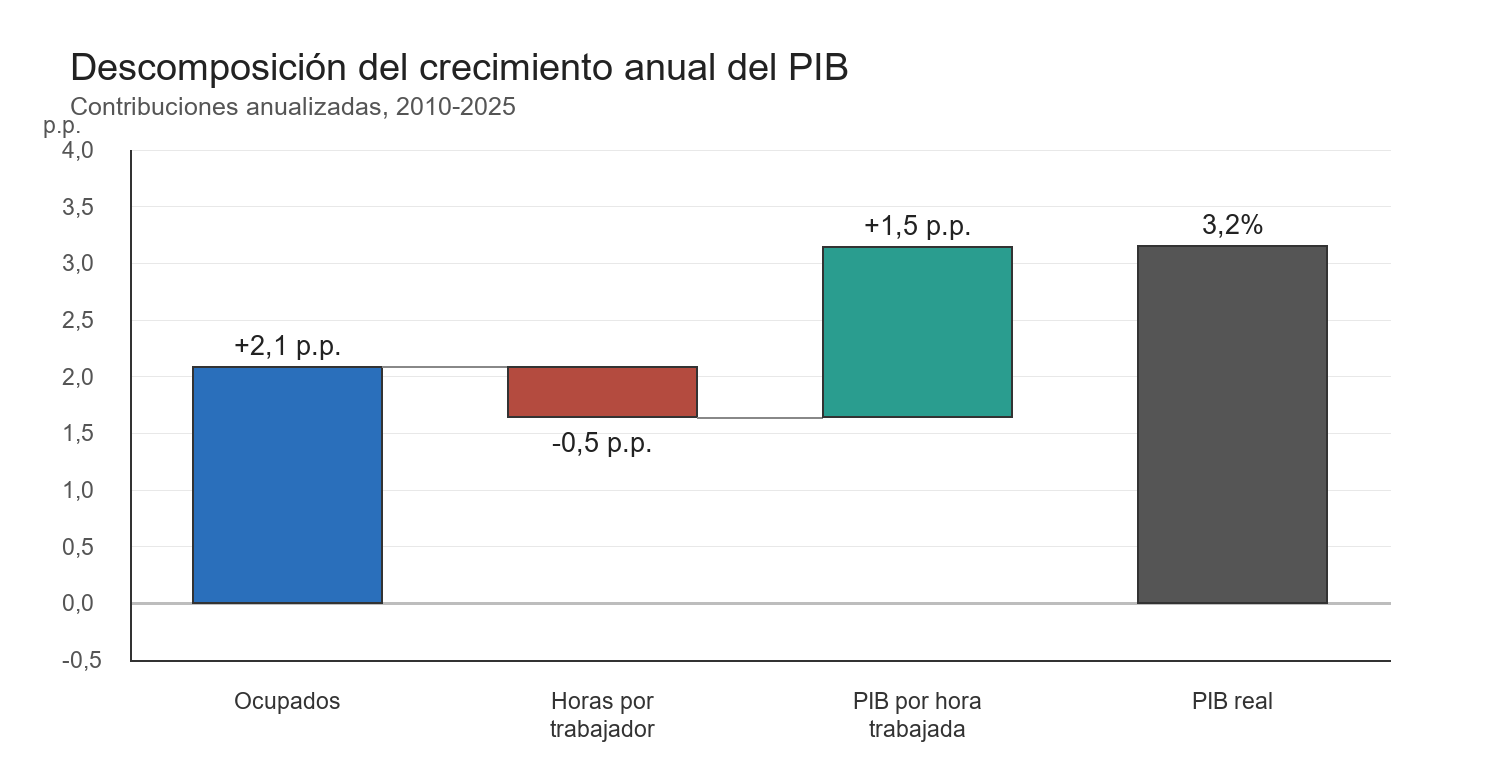
\includegraphics[width=0.82\textwidth]{fig_pib_geih_descomposicion_crecimiento_comunicado.png}
  \caption{Descomposición del crecimiento anual del PIB, 2010--2025}
  \label{fig:comunicado_descomposicion}
  \caption*{Nota: las barras intermedias muestran cuánto aporta cada componente, en puntos porcentuales, al crecimiento anualizado del PIB real. Fuente: cálculos propios con base en Cuentas Nacionales y GEIH del DANE.}
\end{figure}

\begin{table}[H]
\centering
\caption{Productividad laboral por actividad económica, 2010--2025}
\label{tab:comunicado_productividad_sector}
\setlength{\tabcolsep}{4pt}
\begin{tabular}{>{\raggedright\arraybackslash}p{5.4cm}rrrrrr}
\toprule
& \multicolumn{3}{c}{PIB por trabajador} & \multicolumn{3}{c}{PIB por hora} \\
& \multicolumn{3}{c}{Millones de pesos de 2015} & \multicolumn{3}{c}{Miles de pesos de 2015} \\
\cmidrule(lr){2-4}\cmidrule(lr){5-7}
Actividad económica & 2010 & 2025 & Crec. & 2010 & 2025 & Crec. \\
\midrule
Arte, recreación y otros servicios & 11,4 & 32,8 & 7,3\% & 5,6 & 16,0 & 7,3\% \\
Información y comunicaciones & 45,4 & 78,6 & 3,7\% & 17,6 & 34,0 & 4,5\% \\
Agropecuario & 13,5 & 20,4 & 2,8\% & 5,8 & 9,4 & 3,3\% \\
Hogares como empleadores & 6,4 & 9,4 & 2,6\% & 2,7 & 4,5 & 3,5\% \\
Adm. pública, educación y salud & 43,9 & 58,4 & 1,9\% & 19,5 & 26,1 & 2,0\% \\
Financieras & 101,0 & 124,5 & 1,4\% & 43,0 & 54,2 & 1,6\% \\
Comercio, transporte y alojamiento & 20,9 & 24,1 & 1,0\% & 7,9 & 10,1 & 1,6\% \\
Manufactura & 40,1 & 45,0 & 0,8\% & 16,5 & 19,5 & 1,1\% \\
Inmobiliarias & 280,0 & 284,6 & 0,1\% & 105,3 & 119,5 & 0,9\% \\
Profesionales y administrativas & 54,3 & 42,4 & -1,6\% & 24,8 & 20,6 & -1,2\% \\
Construcción & 41,8 & 26,1 & -3,1\% & 16,4 & 11,0 & -2,6\% \\
Minas & 200,8 & 115,8 & -3,6\% & 77,6 & 48,4 & -3,1\% \\
Servicios públicos & 176,5 & 99,5 & -3,8\% & 70,0 & 43,5 & -3,1\% \\
\bottomrule
\end{tabular}
\caption*{Nota: las actividades están ordenadas por el crecimiento anual del PIB por trabajador. Fuente: cálculos propios con DANE y GEIH.}
\end{table}

{\color{cjcblue}\rule{\textwidth}{0.6pt}}

\end{document}
